% =====================================================================
%  fig/fig_architecture.tex -- the MoRE block diagram, drawn in pure TikZ.
%
%  WHY TIKZ AND NOT A PNG. Vector output at any zoom, matches the ACL
%  typeface exactly, needs no external file, and is editable as text -- so
%  a reviewer-requested tweak is a one-line change rather than a redraw.
%
%  HOW TO USE IN OVERLEAF
%  1. In main.tex's preamble (after \usepackage{graphicx}) add exactly:
%         \usepackage{tikz}
%     No \usetikzlibrary line is needed: this file uses only core TikZ
%     (rounded corners, fills, plain -> arrows, -- and |- paths).
%  2. In sections/02_method.tex, replace the whole
%         \begin{figure*} ... \end{figure*}
%     block that currently 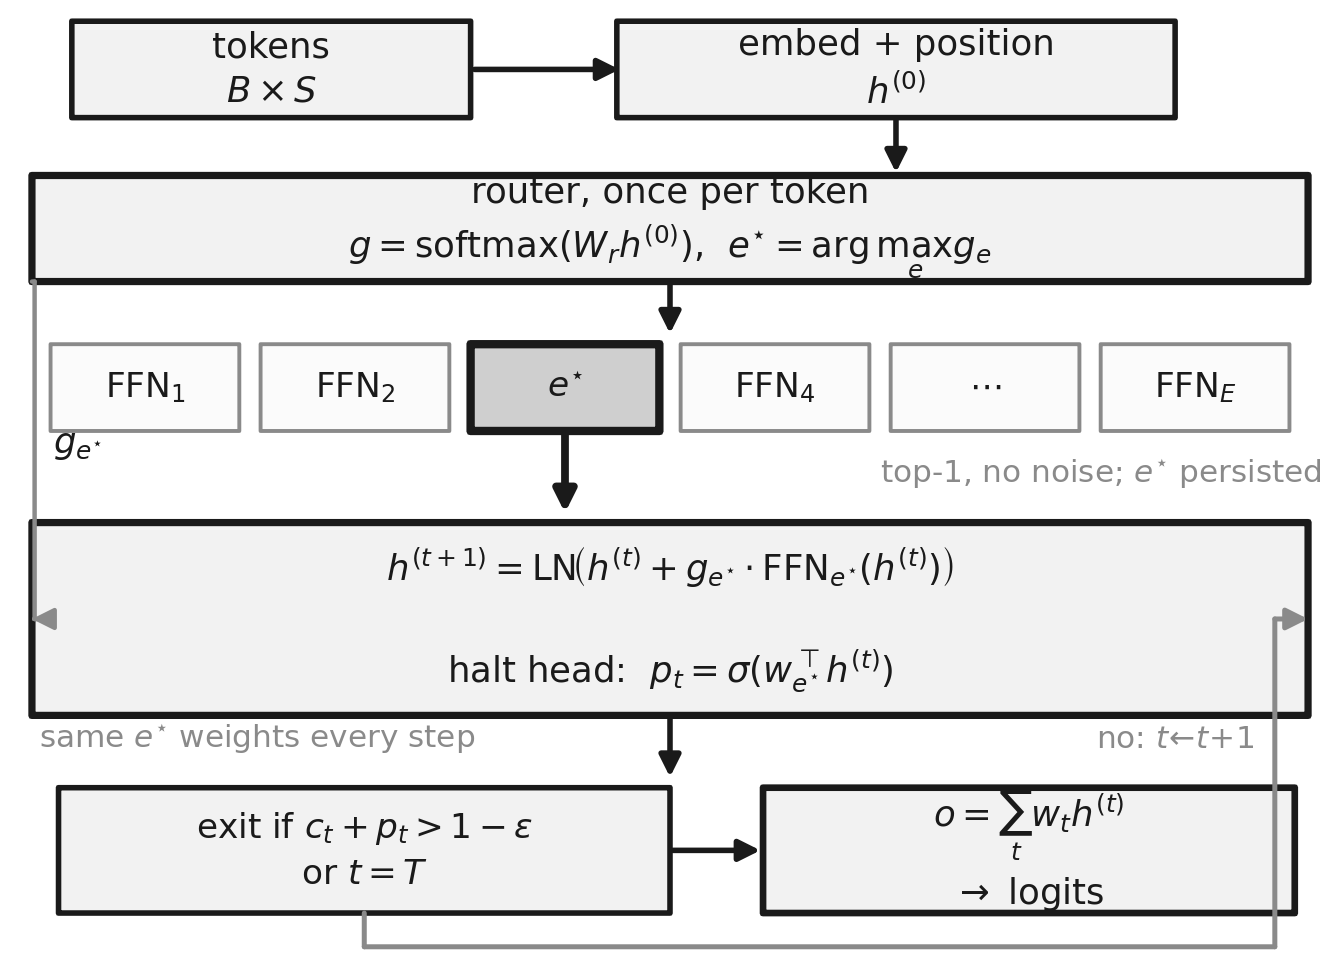
\includegraphics{fig_architecture.png} with the
%     single line:
%         % =====================================================================
%  fig/fig_architecture.tex -- the MoRE block diagram, drawn in pure TikZ.
%
%  WHY TIKZ AND NOT A PNG. Vector output at any zoom, matches the ACL
%  typeface exactly, needs no external file, and is editable as text -- so
%  a reviewer-requested tweak is a one-line change rather than a redraw.
%
%  HOW TO USE IN OVERLEAF
%  1. In main.tex's preamble (after \usepackage{graphicx}) add exactly:
%         \usepackage{tikz}
%     No \usetikzlibrary line is needed: this file uses only core TikZ
%     (rounded corners, fills, plain -> arrows, -- and |- paths).
%  2. In sections/02_method.tex, replace the whole
%         \begin{figure*} ... \end{figure*}
%     block that currently 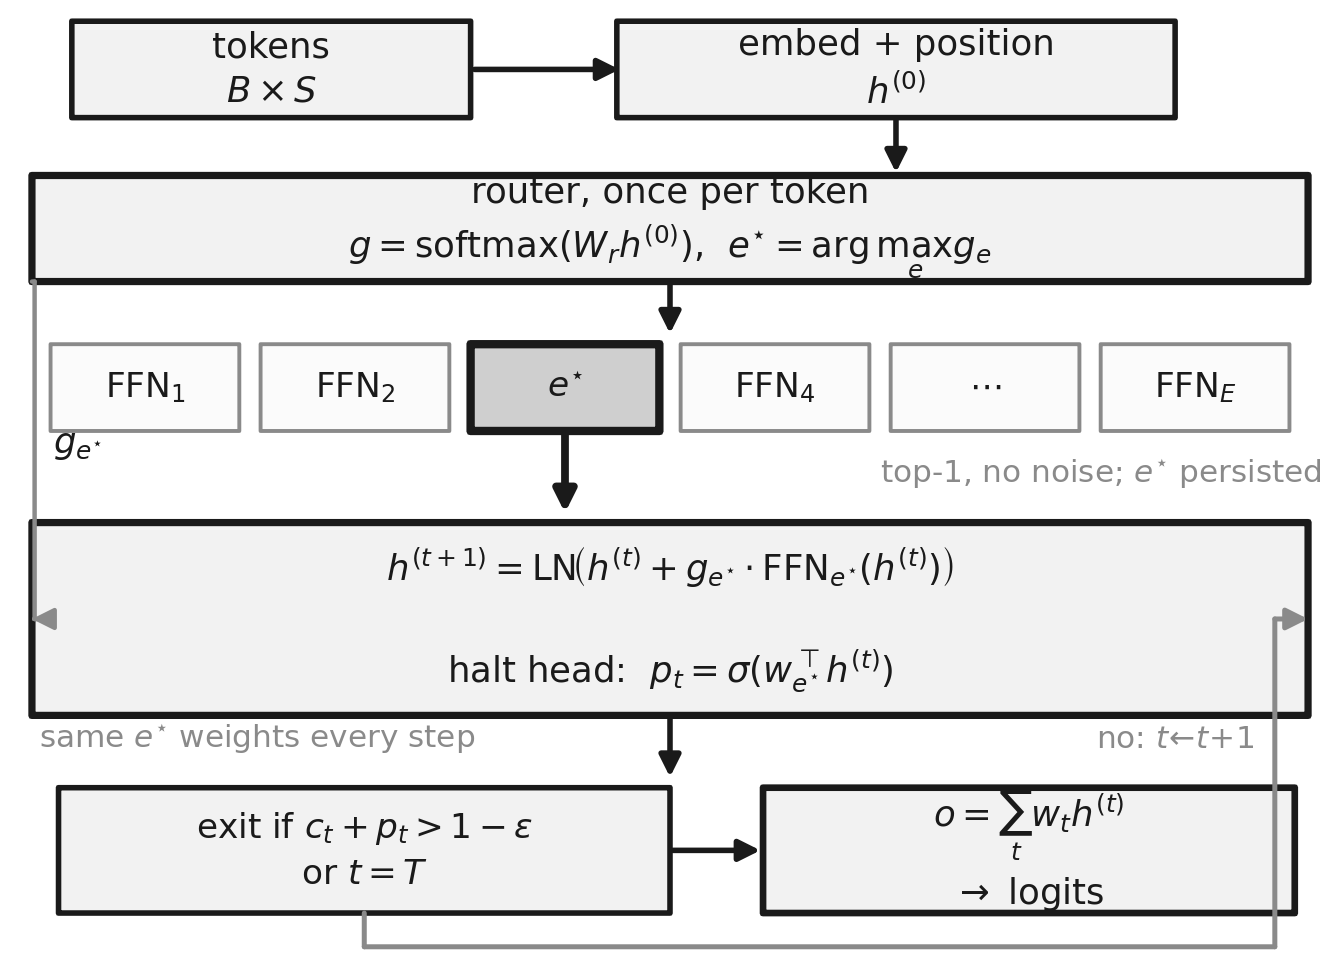
\includegraphics{fig_architecture.png} with the
%     single line:
%         % =====================================================================
%  fig/fig_architecture.tex -- the MoRE block diagram, drawn in pure TikZ.
%
%  WHY TIKZ AND NOT A PNG. Vector output at any zoom, matches the ACL
%  typeface exactly, needs no external file, and is editable as text -- so
%  a reviewer-requested tweak is a one-line change rather than a redraw.
%
%  HOW TO USE IN OVERLEAF
%  1. In main.tex's preamble (after \usepackage{graphicx}) add exactly:
%         \usepackage{tikz}
%     No \usetikzlibrary line is needed: this file uses only core TikZ
%     (rounded corners, fills, plain -> arrows, -- and |- paths).
%  2. In sections/02_method.tex, replace the whole
%         \begin{figure*} ... \end{figure*}
%     block that currently 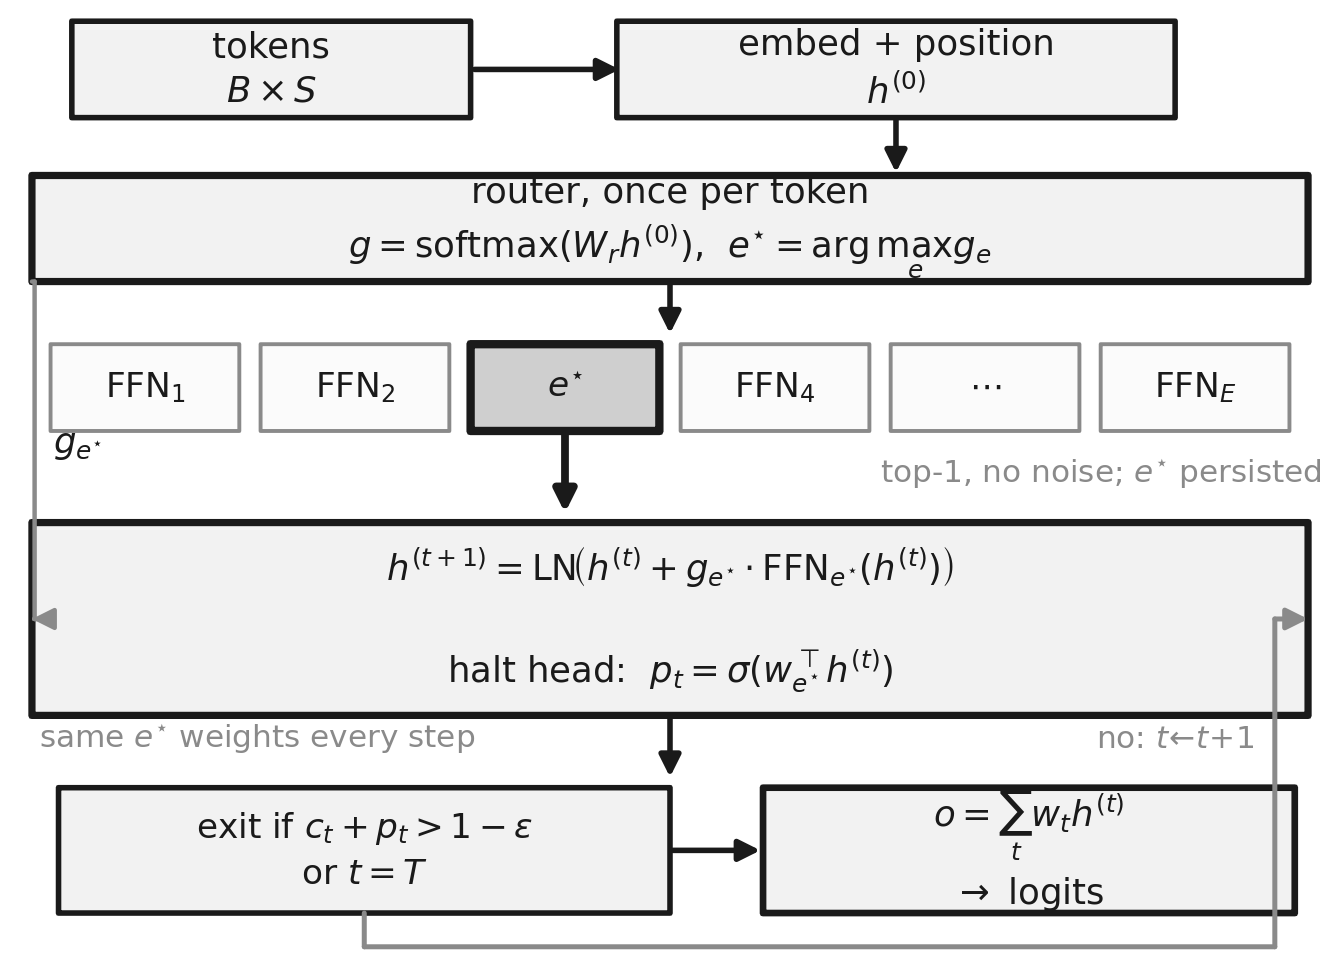
\includegraphics{fig_architecture.png} with the
%     single line:
%         % =====================================================================
%  fig/fig_architecture.tex -- the MoRE block diagram, drawn in pure TikZ.
%
%  WHY TIKZ AND NOT A PNG. Vector output at any zoom, matches the ACL
%  typeface exactly, needs no external file, and is editable as text -- so
%  a reviewer-requested tweak is a one-line change rather than a redraw.
%
%  HOW TO USE IN OVERLEAF
%  1. In main.tex's preamble (after \usepackage{graphicx}) add exactly:
%         \usepackage{tikz}
%     No \usetikzlibrary line is needed: this file uses only core TikZ
%     (rounded corners, fills, plain -> arrows, -- and |- paths).
%  2. In sections/02_method.tex, replace the whole
%         \begin{figure*} ... \end{figure*}
%     block that currently 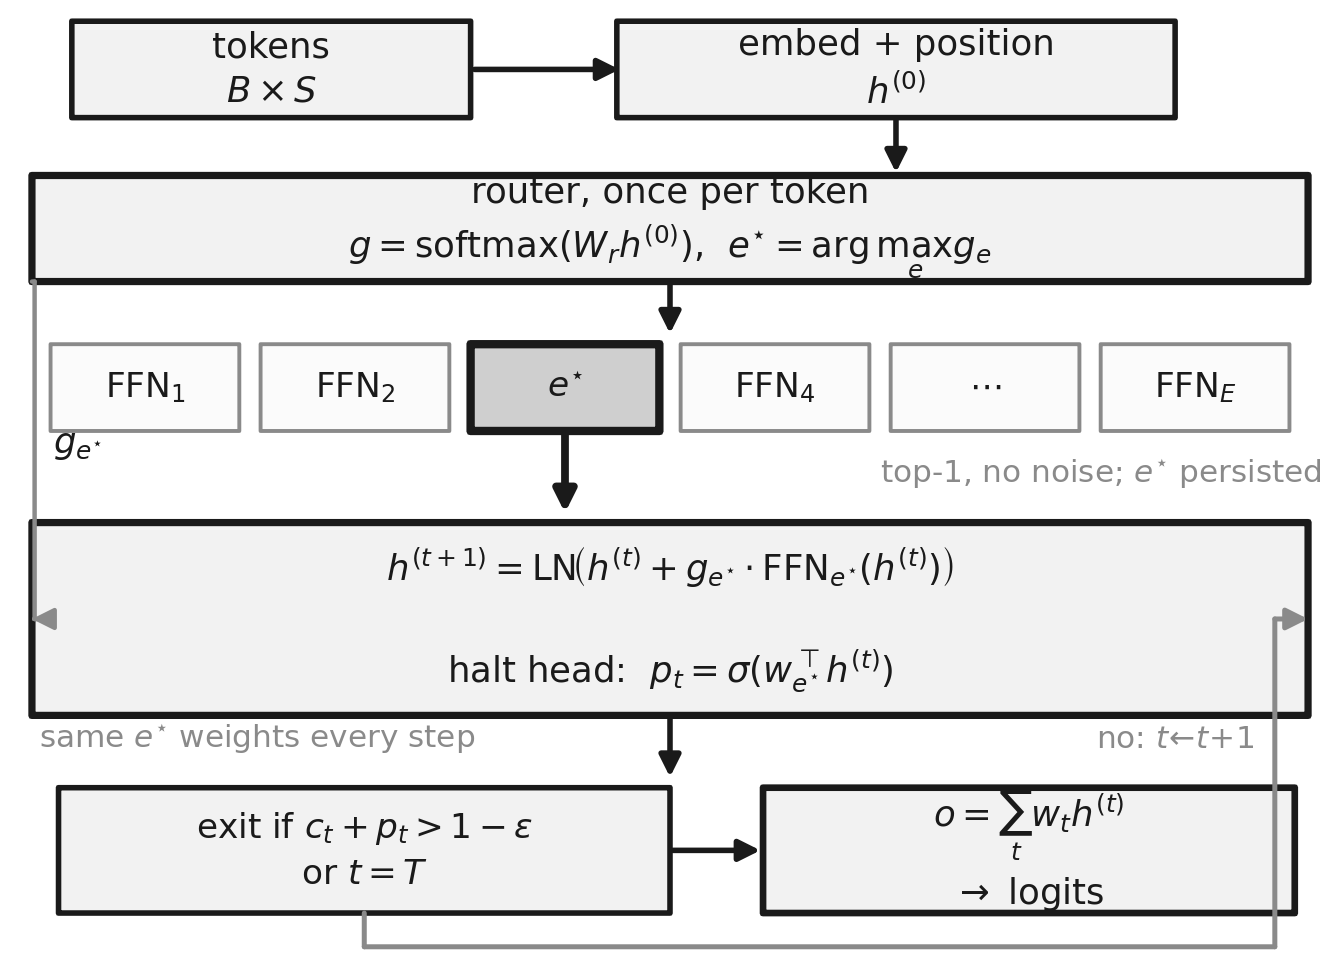
\includegraphics{fig_architecture.png} with the
%     single line:
%         \input{fig/fig_architecture}
%  3. Rebuild. Delete fig_architecture.png only once this compiles.
%
%  WHAT THE DIAGRAM ENCODES, and why each element is there (the code is the
%  authority; this is the reading):
%    * routing happens ONCE, from the post-embedding state h^(0) -- the
%      token is assigned e* before any recursion, and keeps it for the whole
%      trajectory (this is the route-once specification, T-LX.12);
%    * only the selected expert is evaluated (top-1 sparse), and its output
%      is scaled by the gate g_{e*};
%    * the SAME expert weights are reused at every depth step (weight tying)
%      -- the block formula is Eq. (1) of the paper;
%    * a per-expert halt head emits p_t at each step (Eq. 2);
%    * the loop recurses until c_t + p_t > 1-eps, with a forced exit at t=T
%      (Eq. 3), and the output is the convex combination sum_t w_t h^(t);
%    * T=1 recovers MoE and E=1 recovers MoR, which is what makes the three
%      arms configurations of one engine rather than three models.
% =====================================================================
\begin{figure*}[t]
\centering
\resizebox{0.98\linewidth}{!}{%
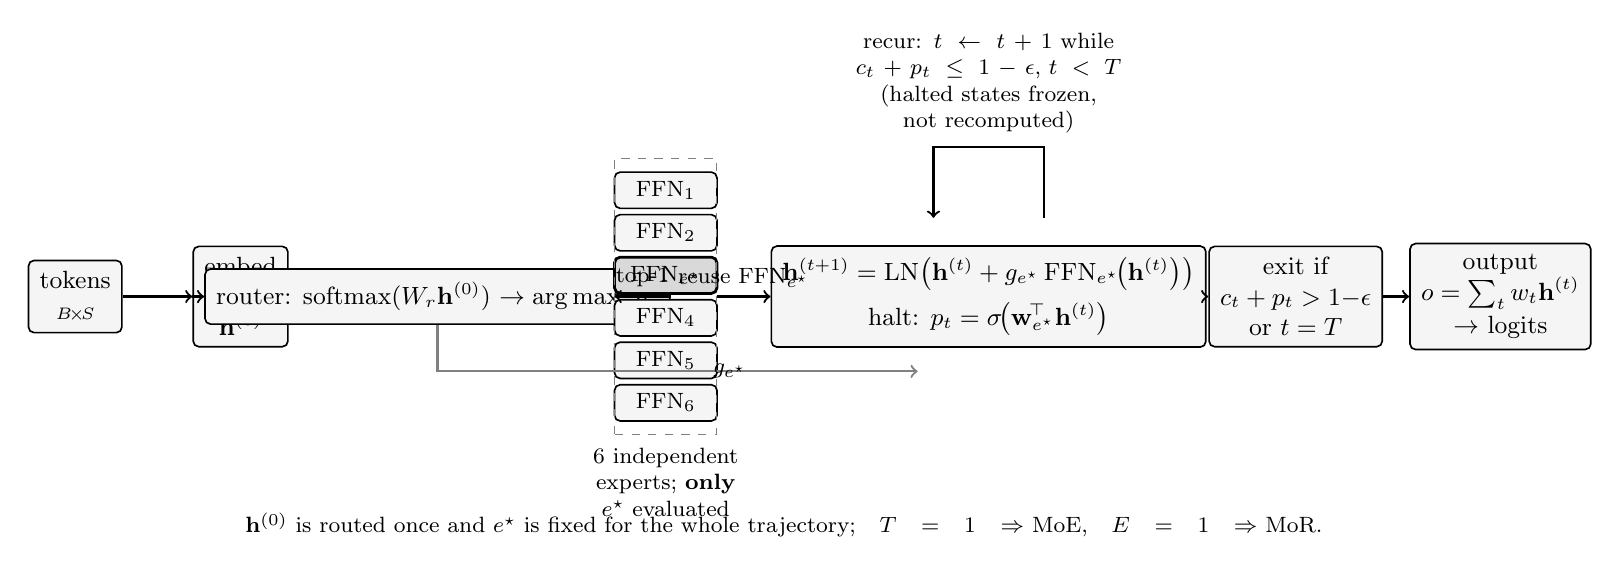
\begin{tikzpicture}[font=\small]
  \tikzset{
    box/.style   = {draw, rounded corners=2pt, align=center, inner sep=4pt,
                    minimum height=7mm, line width=0.6pt},
    st/.style    = {box, fill=black!4},
    ex/.style    = {box, fill=black!4, minimum width=13mm,
                    minimum height=4.6mm, inner sep=1.5pt, font=\footnotesize},
    sel/.style   = {box, fill=black!15, minimum width=13mm,
                    minimum height=4.6mm, inner sep=1.5pt, font=\footnotesize,
                    line width=1.0pt},
    nb/.style    = {font=\footnotesize, align=center, inner sep=2pt},
    ar/.style    = {->, thick}
  }

  % ---------- main axis: tokens -> embed -> router ----------
  \node[st] (tok) at (0.0,0) {tokens\\ $\scriptstyle B\!\times\!S$};
  \node[st] (emb) at (2.1,0) {embed\\ $+$ pos\\ $\mathbf{h}^{(0)}$};
  \node[st] (rtr) at (4.6,0) {router: $\mathrm{softmax}(W_r\mathbf{h}^{(0)})$
        $\to \arg\max_e g_e$};

  % ---------- the expert bank: six FFNs, only e* evaluated ----------
  \foreach \i in {1,...,6} {
    \pgfmathsetmacro{\yy}{1.35 - 0.54*(\i-1)}
    \ifnum\i=3
      \node[sel] (e\i) at (7.5,\yy) {FFN$_{e^\star}$};
    \else
      \node[ex]  (e\i) at (7.5,\yy) {FFN$_{\i}$};
    \fi
  }
  \draw[dashed, gray] (6.85,-1.75) rectangle (8.15,1.75);
  \node[nb, anchor=north, text width=28mm] at (7.5,-1.85)
       {6 independent experts; \textbf{only} $e^\star$ evaluated};

  % ---------- the tied recursion block (Eq. 1 + Eq. 2) ----------
  \node[st, minimum width=42mm] (rec) at (11.6,0)
       {$\mathbf{h}^{(t+1)}=\mathrm{LN}\!\left(
          \mathbf{h}^{(t)} + g_{e^\star}\,\mathrm{FFN}_{e^\star}\!\big(\mathbf{h}^{(t)}\big)
        \right)$\\[3pt]
        halt: $p_t=\sigma\!\big(\mathbf{w}_{e^\star}^{\!\top}\mathbf{h}^{(t)}\big)$};

  % ---------- exit decision (Eq. 3) and output ----------
  \node[st] (exit) at (15.5,0) {exit if\\ $c_t+p_t>1{-}\epsilon$\\ or $t=T$};
  \node[st] (out)  at (18.1,0) {output\\ $o=\sum_t w_t\mathbf{h}^{(t)}$\\[1pt]
                                 $\to$ logits};

  % ---------- main-path arrows ----------
  \draw[ar] (tok) -- (emb);
  \draw[ar] (emb) -- (rtr);
  \draw[ar] (rtr.east) -- (6.85,0)
        node[midway, above=1pt, nb] {top-1};
  \draw[ar] (8.15,0) -- (rec.west)
        node[midway, above=1pt, nb] {reuse $\mathrm{FFN}_{e^\star}$};
  \draw[ar] (rec) -- (exit);
  \draw[ar] (exit) -- (out);

  % the gate multiplies the expert output
  \draw[ar, gray] (rtr.south) |- (10.7,-0.95)
        node[pos=0.78, right, nb, text=black] {$g_{e^\star}$};

  % ---------- the recursion self-loop ----------
  \draw[ar] (12.3,1.0) -- (12.3,1.9) -- (10.9,1.9) -- (10.9,1.0);
  \node[nb, anchor=south, text width=48mm] at (11.6,2.0)
       {recur: $t \leftarrow t+1$ while $c_t+p_t\le 1-\epsilon$,\ $t<T$\\
        (halted states frozen, not recomputed)};

  % ---------- bottom note ----------
  \node[nb, text width=170mm] at (9.0,-2.9)
       {$\mathbf{h}^{(0)}$ is routed once and $e^\star$ is fixed for the whole
        trajectory;\quad $T=1\Rightarrow$ MoE,\quad $E=1\Rightarrow$ MoR.};

\end{tikzpicture}}
\caption{The MoRE block, drawn in TikZ. A token is routed \emph{once} from its
post-embedding state to one of $E$ independent expert FFNs, and \emph{that
expert's} weights---never another's---are reused for an adaptive number of
recursion steps under ACT halting. Only the selected expert is evaluated, and
its output is scaled by the gate $g_{e^\star}$. Setting $T=1$ recovers MoE
exactly and setting $E=1$ recovers MoR; the input representation is bit-identical
in all three cases, and all three are configurations of one engine.}
\label{fig:architecture}
\end{figure*}


%  3. Rebuild. Delete fig_architecture.png only once this compiles.
%
%  WHAT THE DIAGRAM ENCODES, and why each element is there (the code is the
%  authority; this is the reading):
%    * routing happens ONCE, from the post-embedding state h^(0) -- the
%      token is assigned e* before any recursion, and keeps it for the whole
%      trajectory (this is the route-once specification, T-LX.12);
%    * only the selected expert is evaluated (top-1 sparse), and its output
%      is scaled by the gate g_{e*};
%    * the SAME expert weights are reused at every depth step (weight tying)
%      -- the block formula is Eq. (1) of the paper;
%    * a per-expert halt head emits p_t at each step (Eq. 2);
%    * the loop recurses until c_t + p_t > 1-eps, with a forced exit at t=T
%      (Eq. 3), and the output is the convex combination sum_t w_t h^(t);
%    * T=1 recovers MoE and E=1 recovers MoR, which is what makes the three
%      arms configurations of one engine rather than three models.
% =====================================================================
\begin{figure*}[t]
\centering
\resizebox{0.98\linewidth}{!}{%
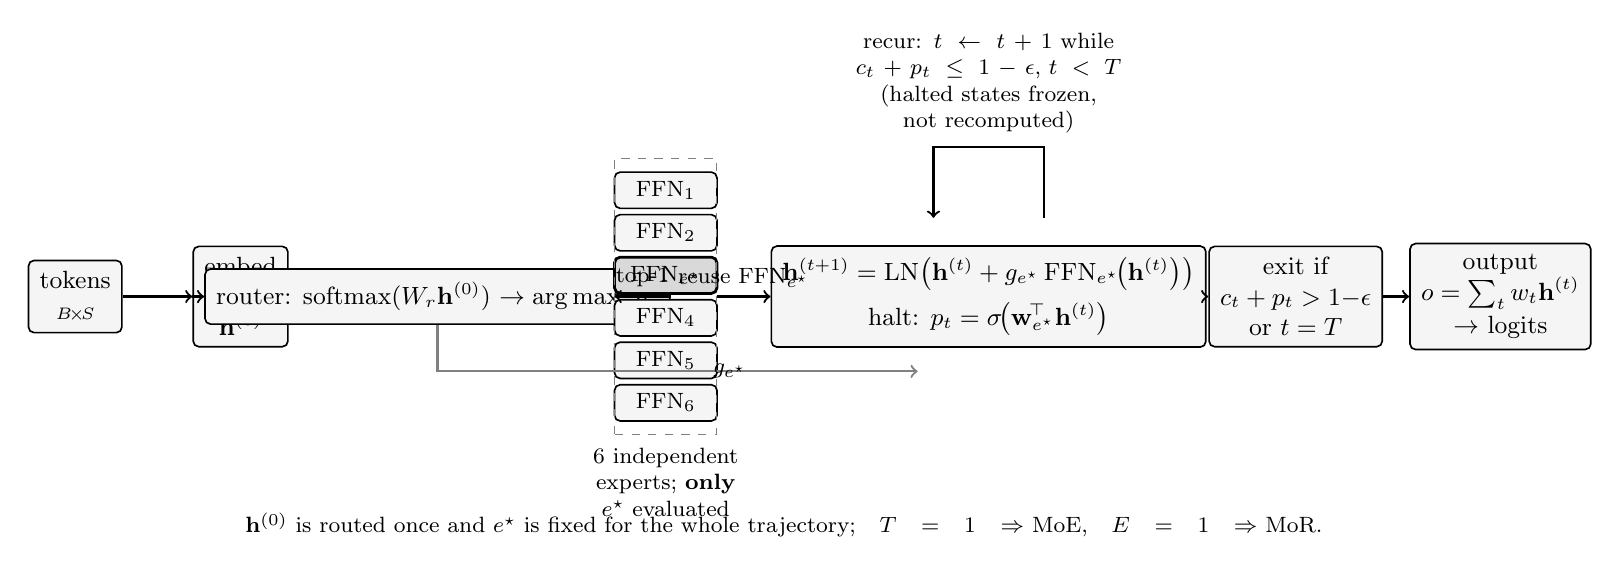
\begin{tikzpicture}[font=\small]
  \tikzset{
    box/.style   = {draw, rounded corners=2pt, align=center, inner sep=4pt,
                    minimum height=7mm, line width=0.6pt},
    st/.style    = {box, fill=black!4},
    ex/.style    = {box, fill=black!4, minimum width=13mm,
                    minimum height=4.6mm, inner sep=1.5pt, font=\footnotesize},
    sel/.style   = {box, fill=black!15, minimum width=13mm,
                    minimum height=4.6mm, inner sep=1.5pt, font=\footnotesize,
                    line width=1.0pt},
    nb/.style    = {font=\footnotesize, align=center, inner sep=2pt},
    ar/.style    = {->, thick}
  }

  % ---------- main axis: tokens -> embed -> router ----------
  \node[st] (tok) at (0.0,0) {tokens\\ $\scriptstyle B\!\times\!S$};
  \node[st] (emb) at (2.1,0) {embed\\ $+$ pos\\ $\mathbf{h}^{(0)}$};
  \node[st] (rtr) at (4.6,0) {router: $\mathrm{softmax}(W_r\mathbf{h}^{(0)})$
        $\to \arg\max_e g_e$};

  % ---------- the expert bank: six FFNs, only e* evaluated ----------
  \foreach \i in {1,...,6} {
    \pgfmathsetmacro{\yy}{1.35 - 0.54*(\i-1)}
    \ifnum\i=3
      \node[sel] (e\i) at (7.5,\yy) {FFN$_{e^\star}$};
    \else
      \node[ex]  (e\i) at (7.5,\yy) {FFN$_{\i}$};
    \fi
  }
  \draw[dashed, gray] (6.85,-1.75) rectangle (8.15,1.75);
  \node[nb, anchor=north, text width=28mm] at (7.5,-1.85)
       {6 independent experts; \textbf{only} $e^\star$ evaluated};

  % ---------- the tied recursion block (Eq. 1 + Eq. 2) ----------
  \node[st, minimum width=42mm] (rec) at (11.6,0)
       {$\mathbf{h}^{(t+1)}=\mathrm{LN}\!\left(
          \mathbf{h}^{(t)} + g_{e^\star}\,\mathrm{FFN}_{e^\star}\!\big(\mathbf{h}^{(t)}\big)
        \right)$\\[3pt]
        halt: $p_t=\sigma\!\big(\mathbf{w}_{e^\star}^{\!\top}\mathbf{h}^{(t)}\big)$};

  % ---------- exit decision (Eq. 3) and output ----------
  \node[st] (exit) at (15.5,0) {exit if\\ $c_t+p_t>1{-}\epsilon$\\ or $t=T$};
  \node[st] (out)  at (18.1,0) {output\\ $o=\sum_t w_t\mathbf{h}^{(t)}$\\[1pt]
                                 $\to$ logits};

  % ---------- main-path arrows ----------
  \draw[ar] (tok) -- (emb);
  \draw[ar] (emb) -- (rtr);
  \draw[ar] (rtr.east) -- (6.85,0)
        node[midway, above=1pt, nb] {top-1};
  \draw[ar] (8.15,0) -- (rec.west)
        node[midway, above=1pt, nb] {reuse $\mathrm{FFN}_{e^\star}$};
  \draw[ar] (rec) -- (exit);
  \draw[ar] (exit) -- (out);

  % the gate multiplies the expert output
  \draw[ar, gray] (rtr.south) |- (10.7,-0.95)
        node[pos=0.78, right, nb, text=black] {$g_{e^\star}$};

  % ---------- the recursion self-loop ----------
  \draw[ar] (12.3,1.0) -- (12.3,1.9) -- (10.9,1.9) -- (10.9,1.0);
  \node[nb, anchor=south, text width=48mm] at (11.6,2.0)
       {recur: $t \leftarrow t+1$ while $c_t+p_t\le 1-\epsilon$,\ $t<T$\\
        (halted states frozen, not recomputed)};

  % ---------- bottom note ----------
  \node[nb, text width=170mm] at (9.0,-2.9)
       {$\mathbf{h}^{(0)}$ is routed once and $e^\star$ is fixed for the whole
        trajectory;\quad $T=1\Rightarrow$ MoE,\quad $E=1\Rightarrow$ MoR.};

\end{tikzpicture}}
\caption{The MoRE block, drawn in TikZ. A token is routed \emph{once} from its
post-embedding state to one of $E$ independent expert FFNs, and \emph{that
expert's} weights---never another's---are reused for an adaptive number of
recursion steps under ACT halting. Only the selected expert is evaluated, and
its output is scaled by the gate $g_{e^\star}$. Setting $T=1$ recovers MoE
exactly and setting $E=1$ recovers MoR; the input representation is bit-identical
in all three cases, and all three are configurations of one engine.}
\label{fig:architecture}
\end{figure*}


%  3. Rebuild. Delete fig_architecture.png only once this compiles.
%
%  WHAT THE DIAGRAM ENCODES, and why each element is there (the code is the
%  authority; this is the reading):
%    * routing happens ONCE, from the post-embedding state h^(0) -- the
%      token is assigned e* before any recursion, and keeps it for the whole
%      trajectory (this is the route-once specification, T-LX.12);
%    * only the selected expert is evaluated (top-1 sparse), and its output
%      is scaled by the gate g_{e*};
%    * the SAME expert weights are reused at every depth step (weight tying)
%      -- the block formula is Eq. (1) of the paper;
%    * a per-expert halt head emits p_t at each step (Eq. 2);
%    * the loop recurses until c_t + p_t > 1-eps, with a forced exit at t=T
%      (Eq. 3), and the output is the convex combination sum_t w_t h^(t);
%    * T=1 recovers MoE and E=1 recovers MoR, which is what makes the three
%      arms configurations of one engine rather than three models.
% =====================================================================
\begin{figure*}[t]
\centering
\resizebox{0.98\linewidth}{!}{%
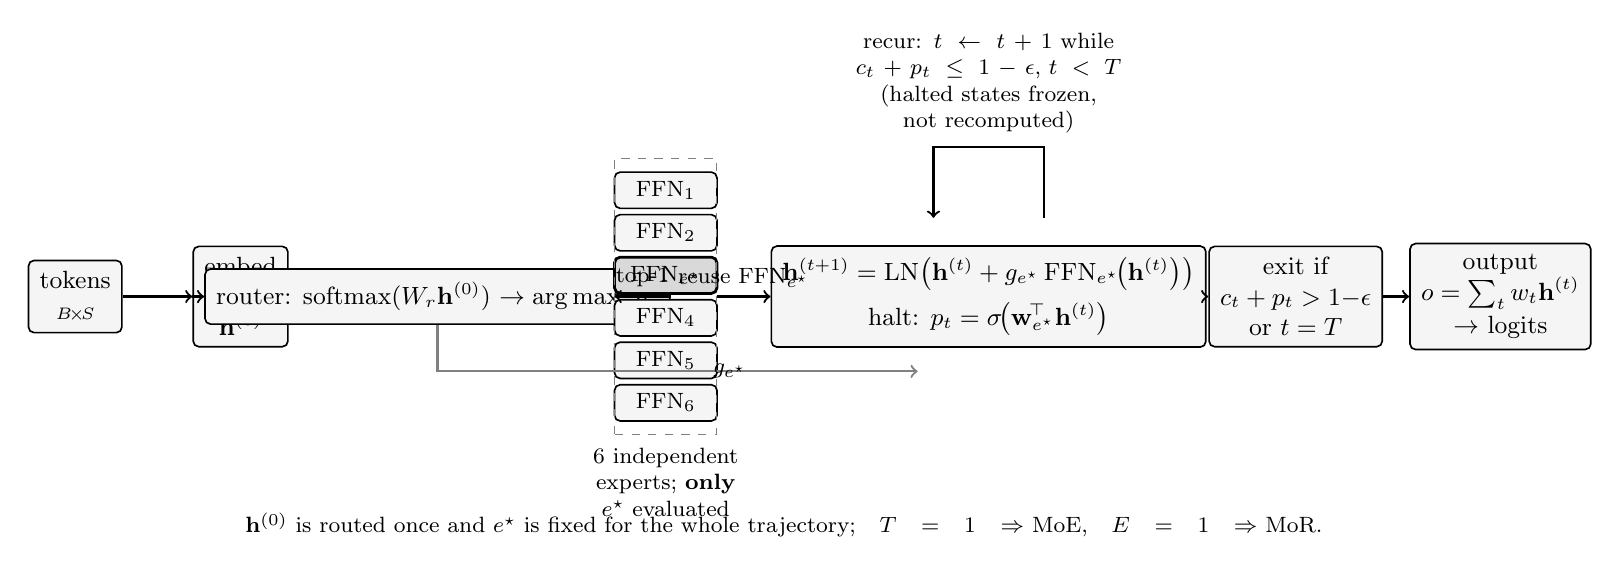
\begin{tikzpicture}[font=\small]
  \tikzset{
    box/.style   = {draw, rounded corners=2pt, align=center, inner sep=4pt,
                    minimum height=7mm, line width=0.6pt},
    st/.style    = {box, fill=black!4},
    ex/.style    = {box, fill=black!4, minimum width=13mm,
                    minimum height=4.6mm, inner sep=1.5pt, font=\footnotesize},
    sel/.style   = {box, fill=black!15, minimum width=13mm,
                    minimum height=4.6mm, inner sep=1.5pt, font=\footnotesize,
                    line width=1.0pt},
    nb/.style    = {font=\footnotesize, align=center, inner sep=2pt},
    ar/.style    = {->, thick}
  }

  % ---------- main axis: tokens -> embed -> router ----------
  \node[st] (tok) at (0.0,0) {tokens\\ $\scriptstyle B\!\times\!S$};
  \node[st] (emb) at (2.1,0) {embed\\ $+$ pos\\ $\mathbf{h}^{(0)}$};
  \node[st] (rtr) at (4.6,0) {router: $\mathrm{softmax}(W_r\mathbf{h}^{(0)})$
        $\to \arg\max_e g_e$};

  % ---------- the expert bank: six FFNs, only e* evaluated ----------
  \foreach \i in {1,...,6} {
    \pgfmathsetmacro{\yy}{1.35 - 0.54*(\i-1)}
    \ifnum\i=3
      \node[sel] (e\i) at (7.5,\yy) {FFN$_{e^\star}$};
    \else
      \node[ex]  (e\i) at (7.5,\yy) {FFN$_{\i}$};
    \fi
  }
  \draw[dashed, gray] (6.85,-1.75) rectangle (8.15,1.75);
  \node[nb, anchor=north, text width=28mm] at (7.5,-1.85)
       {6 independent experts; \textbf{only} $e^\star$ evaluated};

  % ---------- the tied recursion block (Eq. 1 + Eq. 2) ----------
  \node[st, minimum width=42mm] (rec) at (11.6,0)
       {$\mathbf{h}^{(t+1)}=\mathrm{LN}\!\left(
          \mathbf{h}^{(t)} + g_{e^\star}\,\mathrm{FFN}_{e^\star}\!\big(\mathbf{h}^{(t)}\big)
        \right)$\\[3pt]
        halt: $p_t=\sigma\!\big(\mathbf{w}_{e^\star}^{\!\top}\mathbf{h}^{(t)}\big)$};

  % ---------- exit decision (Eq. 3) and output ----------
  \node[st] (exit) at (15.5,0) {exit if\\ $c_t+p_t>1{-}\epsilon$\\ or $t=T$};
  \node[st] (out)  at (18.1,0) {output\\ $o=\sum_t w_t\mathbf{h}^{(t)}$\\[1pt]
                                 $\to$ logits};

  % ---------- main-path arrows ----------
  \draw[ar] (tok) -- (emb);
  \draw[ar] (emb) -- (rtr);
  \draw[ar] (rtr.east) -- (6.85,0)
        node[midway, above=1pt, nb] {top-1};
  \draw[ar] (8.15,0) -- (rec.west)
        node[midway, above=1pt, nb] {reuse $\mathrm{FFN}_{e^\star}$};
  \draw[ar] (rec) -- (exit);
  \draw[ar] (exit) -- (out);

  % the gate multiplies the expert output
  \draw[ar, gray] (rtr.south) |- (10.7,-0.95)
        node[pos=0.78, right, nb, text=black] {$g_{e^\star}$};

  % ---------- the recursion self-loop ----------
  \draw[ar] (12.3,1.0) -- (12.3,1.9) -- (10.9,1.9) -- (10.9,1.0);
  \node[nb, anchor=south, text width=48mm] at (11.6,2.0)
       {recur: $t \leftarrow t+1$ while $c_t+p_t\le 1-\epsilon$,\ $t<T$\\
        (halted states frozen, not recomputed)};

  % ---------- bottom note ----------
  \node[nb, text width=170mm] at (9.0,-2.9)
       {$\mathbf{h}^{(0)}$ is routed once and $e^\star$ is fixed for the whole
        trajectory;\quad $T=1\Rightarrow$ MoE,\quad $E=1\Rightarrow$ MoR.};

\end{tikzpicture}}
\caption{The MoRE block, drawn in TikZ. A token is routed \emph{once} from its
post-embedding state to one of $E$ independent expert FFNs, and \emph{that
expert's} weights---never another's---are reused for an adaptive number of
recursion steps under ACT halting. Only the selected expert is evaluated, and
its output is scaled by the gate $g_{e^\star}$. Setting $T=1$ recovers MoE
exactly and setting $E=1$ recovers MoR; the input representation is bit-identical
in all three cases, and all three are configurations of one engine.}
\label{fig:architecture}
\end{figure*}


%  3. Rebuild. Delete fig_architecture.png only once this compiles.
%
%  WHAT THE DIAGRAM ENCODES, and why each element is there (the code is the
%  authority; this is the reading):
%    * routing happens ONCE, from the post-embedding state h^(0) -- the
%      token is assigned e* before any recursion, and keeps it for the whole
%      trajectory (this is the route-once specification, T-LX.12);
%    * only the selected expert is evaluated (top-1 sparse), and its output
%      is scaled by the gate g_{e*};
%    * the SAME expert weights are reused at every depth step (weight tying)
%      -- the block formula is Eq. (1) of the paper;
%    * a per-expert halt head emits p_t at each step (Eq. 2);
%    * the loop recurses until c_t + p_t > 1-eps, with a forced exit at t=T
%      (Eq. 3), and the output is the convex combination sum_t w_t h^(t);
%    * T=1 recovers MoE and E=1 recovers MoR, which is what makes the three
%      arms configurations of one engine rather than three models.
% =====================================================================
\begin{figure*}[t]
\centering
\resizebox{0.98\linewidth}{!}{%
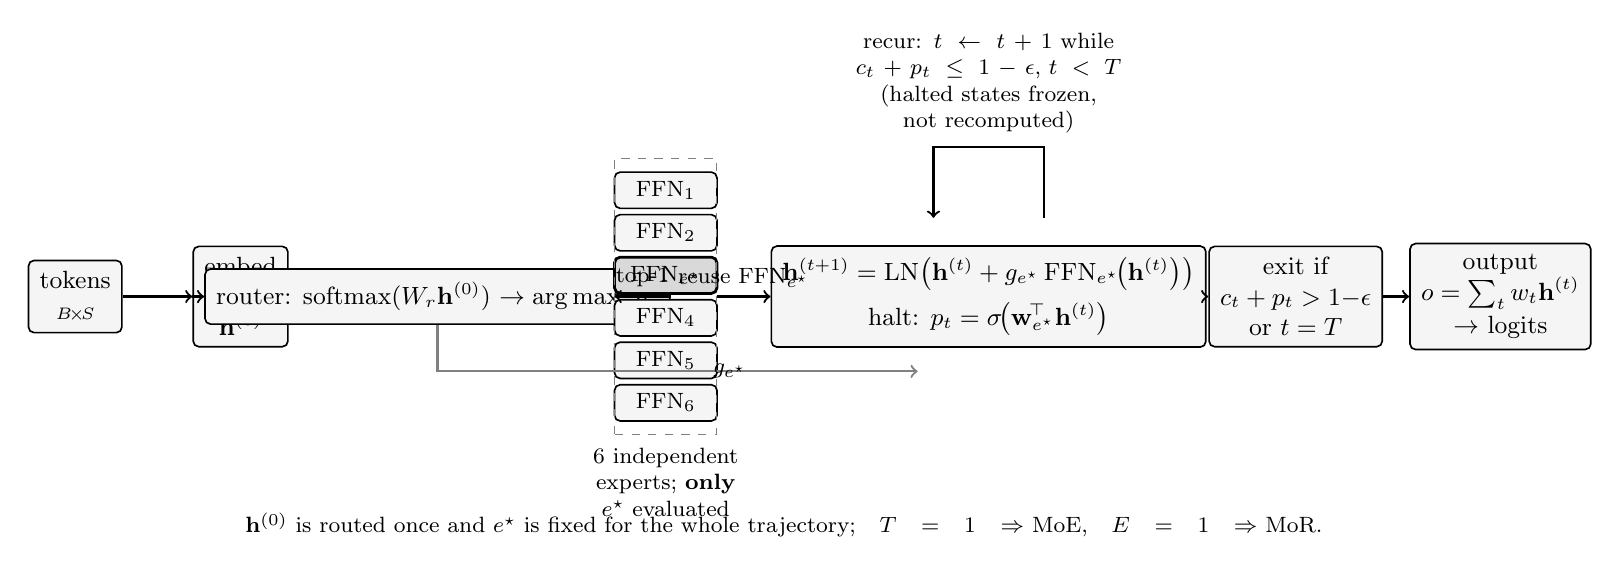
\begin{tikzpicture}[font=\small]
  \tikzset{
    box/.style   = {draw, rounded corners=2pt, align=center, inner sep=4pt,
                    minimum height=7mm, line width=0.6pt},
    st/.style    = {box, fill=black!4},
    ex/.style    = {box, fill=black!4, minimum width=13mm,
                    minimum height=4.6mm, inner sep=1.5pt, font=\footnotesize},
    sel/.style   = {box, fill=black!15, minimum width=13mm,
                    minimum height=4.6mm, inner sep=1.5pt, font=\footnotesize,
                    line width=1.0pt},
    nb/.style    = {font=\footnotesize, align=center, inner sep=2pt},
    ar/.style    = {->, thick}
  }

  % ---------- main axis: tokens -> embed -> router ----------
  \node[st] (tok) at (0.0,0) {tokens\\ $\scriptstyle B\!\times\!S$};
  \node[st] (emb) at (2.1,0) {embed\\ $+$ pos\\ $\mathbf{h}^{(0)}$};
  \node[st] (rtr) at (4.6,0) {router: $\mathrm{softmax}(W_r\mathbf{h}^{(0)})$
        $\to \arg\max_e g_e$};

  % ---------- the expert bank: six FFNs, only e* evaluated ----------
  \foreach \i in {1,...,6} {
    \pgfmathsetmacro{\yy}{1.35 - 0.54*(\i-1)}
    \ifnum\i=3
      \node[sel] (e\i) at (7.5,\yy) {FFN$_{e^\star}$};
    \else
      \node[ex]  (e\i) at (7.5,\yy) {FFN$_{\i}$};
    \fi
  }
  \draw[dashed, gray] (6.85,-1.75) rectangle (8.15,1.75);
  \node[nb, anchor=north, text width=28mm] at (7.5,-1.85)
       {6 independent experts; \textbf{only} $e^\star$ evaluated};

  % ---------- the tied recursion block (Eq. 1 + Eq. 2) ----------
  \node[st, minimum width=42mm] (rec) at (11.6,0)
       {$\mathbf{h}^{(t+1)}=\mathrm{LN}\!\left(
          \mathbf{h}^{(t)} + g_{e^\star}\,\mathrm{FFN}_{e^\star}\!\big(\mathbf{h}^{(t)}\big)
        \right)$\\[3pt]
        halt: $p_t=\sigma\!\big(\mathbf{w}_{e^\star}^{\!\top}\mathbf{h}^{(t)}\big)$};

  % ---------- exit decision (Eq. 3) and output ----------
  \node[st] (exit) at (15.5,0) {exit if\\ $c_t+p_t>1{-}\epsilon$\\ or $t=T$};
  \node[st] (out)  at (18.1,0) {output\\ $o=\sum_t w_t\mathbf{h}^{(t)}$\\[1pt]
                                 $\to$ logits};

  % ---------- main-path arrows ----------
  \draw[ar] (tok) -- (emb);
  \draw[ar] (emb) -- (rtr);
  \draw[ar] (rtr.east) -- (6.85,0)
        node[midway, above=1pt, nb] {top-1};
  \draw[ar] (8.15,0) -- (rec.west)
        node[midway, above=1pt, nb] {reuse $\mathrm{FFN}_{e^\star}$};
  \draw[ar] (rec) -- (exit);
  \draw[ar] (exit) -- (out);

  % the gate multiplies the expert output
  \draw[ar, gray] (rtr.south) |- (10.7,-0.95)
        node[pos=0.78, right, nb, text=black] {$g_{e^\star}$};

  % ---------- the recursion self-loop ----------
  \draw[ar] (12.3,1.0) -- (12.3,1.9) -- (10.9,1.9) -- (10.9,1.0);
  \node[nb, anchor=south, text width=48mm] at (11.6,2.0)
       {recur: $t \leftarrow t+1$ while $c_t+p_t\le 1-\epsilon$,\ $t<T$\\
        (halted states frozen, not recomputed)};

  % ---------- bottom note ----------
  \node[nb, text width=170mm] at (9.0,-2.9)
       {$\mathbf{h}^{(0)}$ is routed once and $e^\star$ is fixed for the whole
        trajectory;\quad $T=1\Rightarrow$ MoE,\quad $E=1\Rightarrow$ MoR.};

\end{tikzpicture}}
\caption{The MoRE block, drawn in TikZ. A token is routed \emph{once} from its
post-embedding state to one of $E$ independent expert FFNs, and \emph{that
expert's} weights---never another's---are reused for an adaptive number of
recursion steps under ACT halting. Only the selected expert is evaluated, and
its output is scaled by the gate $g_{e^\star}$. Setting $T=1$ recovers MoE
exactly and setting $E=1$ recovers MoR; the input representation is bit-identical
in all three cases, and all three are configurations of one engine.}
\label{fig:architecture}
\end{figure*}

